\chapter{Gravity, Free Fall, and Newton's Theorem}

Gravity enters this course as a special force. It is already suspected of having something to do with geometry, but in this first lecture we do not yet develop the general theory of relativity itself. Instead we set up Newtonian gravity in exactly the way that makes the later transition natural: first the Newtonian language of inertial frames, coordinates, and vectors; then the peculiar cancellation of mass in gravitational motion; then the full inverse-square law; and finally the vector calculus that explains why spherical gravitating bodies behave so simply.

\paragraph{Source note.} These companion notes follow Leonard Susskind's first general relativity lecture and preserve its order of argument. This draft was prepared with support from LazyingArt LLC and Video2Book.

\section{Gravity as a Special Force and Newtonian Setup}

Susskind begins by narrowing the scope with some care. Gravity is indeed the road to geometry, but for the moment we work with Newtonian gravity, arranged in a form that will later point toward general relativity. That means we start not with gravity itself, but with Newton's equation of motion.

\begin{definition}
An inertial frame is a coordinate system, equipped with clocks, in which a force-free test object moves with uniform velocity and therefore has zero acceleration.
\end{definition}

The lecture frame preserved below catches the blackboard at the moment when the bare equation \(F=ma\) has just been written. The spoken lecture, however, immediately insists that this is really a vector equation.

\begin{figure}
\centering

\includegraphics[width=0.62\textwidth]{lecture_01_figure_02.png}
\caption{Susskind begins from the stripped-down Newtonian law. The board still shows the scalar handwriting \(F=ma\), but the lecture immediately interprets it as the vector equation \(\vec F = m\vec a\).}
\end{figure}

Thus we write
\begin{align}
\vec F &= m\vec a, \\
F_i &= m a_i = m\ddot x_i, \qquad i=1,2,3.
\end{align}
Here \(m\) is a scalar, not a vector. In Newtonian physics it is an intrinsic and conserved property of the particle. The position of a particle is encoded by its coordinates \(x_1,x_2,x_3\), or equally by the position vector
\begin{equation}
\vec r=(x_1,x_2,x_3).
\end{equation}
Its first time derivative is velocity, and its second time derivative is acceleration:
\begin{equation}
v_i=\dot x_i, \qquad a_i=\ddot x_i.
\end{equation}

This opening is not dead preliminaries. The lecture is preparing a particular comparison. If the force law of gravity turns out to contain the same mass \(m\) that already appears in Newton's law, then something unusual can happen. The mass can cancel, and when it does, the motion becomes universal.

\section{Flat-Earth Gravity and the First Equivalence Principle}

Now Susskind steps even previous to Newton and turns to Galileo's version of gravity. The point is not historical ornament. In the Galilean, or flat-Earth, approximation two simplifications hold at once.

First, the gravitational force points in the same direction everywhere: downward. Second, its magnitude does not depend on height, at least so long as we stay near the Earth's surface and treat the Earth as effectively infinite and flat. If we take the \(x_2\)-direction to be vertical and choose upward as positive, then Galileo's force law becomes
\begin{equation}
F_2=-mg.
\end{equation}
The minus sign records that the force points downward. The constant \(g\) is the near-surface gravitational acceleration; on Earth it is about \(10\,\mathrm{m/s^2}\), but its value depends on the gravitating body and not on the mass of the falling object.

Combining this with Newton's equation gives the first decisive cancellation:
\begin{align}
F_2 &= m\ddot x_2, \\
m\ddot x_2 &= -mg, \\
\ddot x_2 &= -g.
\end{align}
This is the first mathematical signal of the equivalence principle in the lecture. The acceleration of free fall does not depend on the mass of the falling body. A cannonball and a feather, once air resistance is removed from the story, obey the same equation of motion.

What is special about gravity is now visible in a single line. For an electric force, the force is proportional to charge, not mass. For gravity, the force is proportional to precisely the same mass that Newton's equation then places in front of the acceleration. As a result, the motion becomes universal.

\subsection{Question \& Answer}

Why can a freely falling cloud fail to detect gravity even though gravity is present?

Take a diffuse cloud of particles, not even necessarily interacting with one another, and release all of them from rest in the same uniform gravitational field. Because each particle satisfies the same equation \(\ddot x_2=-g\), every particle falls in exactly the same way. Heavy and light particles, large and small particles, all share the same acceleration.

The consequence is stronger than the statement that they all fall. Their relative separations do not change. The cloud does not shear, stretch, or compress. If struts had been holding such an object together, those struts would feel no internal stress from the gravitational field itself. In this flat-Earth approximation, gravity produces no internal deformation.

That is why Susskind says that free fall is locally indistinguishable from being far away from all gravitating bodies. Without the floor, without a tower, and without any external reference, the cloud cannot tell that it is falling. Even the familiar bodily feeling of ``acceleration'' does not contradict this claim. What one ordinarily feels while standing on the Earth is not free fall, but the force of the ground preventing free fall. If that supporting force disappears, one feels strange only because that support has been removed, not because free fall itself is locally detectable in a perfectly uniform field.

This is the lecture's first version of the equivalence principle: uniform gravitational motion is universal, and therefore locally gravity can be hidden by free fall.

\section{Newton's Inverse-Square Law}

The flat-Earth approximation has done its work. We now go beyond it and turn to Newton's full force law. Every object in the universe attracts every other object. Start with two masses, a lighter mass \(m\) and a heavier mass \(M\). Their forces are attractive, equal, and opposite. The magnitude of the force is
\begin{equation}
F=\frac{GmM}{r^2},
\end{equation}
where \(G\) is Newton's constant,
\begin{equation}
G\approx 6.7\times 10^{-11}\,\mathrm{N\,m^2/kg^2}.
\end{equation}

That number is tiny, and the lecture pauses over its smallness. Gravity feels strong in everyday life not because \(G\) is large, but because the Earth is enormous. For two \(1\,\mathrm{kg}\) masses separated by \(1\,\mathrm{m}\),
\begin{equation}
F = G \approx 6.7\times 10^{-11}\,\mathrm N,
\end{equation}
which is far smaller than the easily visible deflections produced by modest electric or magnetic forces.

The blackboard frame below preserves the lecture just before the force law is sharpened into vector form. The board writes the denominator as \(R^2\); in these notes we normalize the notation to \(r=|\vec r|\).

\begin{figure}
\centering

\includegraphics[width=0.72\textwidth]{lecture_01_figure_03.png}
\caption{The lecture first writes the inverse-square law as a statement about magnitude. The point mass \(M\) and the directional sketch on the board prepare the transition to the full vector law.}
\end{figure}

If we place the heavy mass \(M\) at the origin and let \(\vec r\) point from \(M\) to the lighter mass \(m\), then the force on \(m\) must point opposite to \(\vec r\). Introducing the radial unit vector
\begin{equation}
\hat r=\frac{\vec r}{r},
\end{equation}
the vector law becomes
\begin{equation}
\vec F=-\frac{GmM}{r^2}\hat r
      =-\frac{GmM}{r^3}\vec r.
\end{equation}
The extra factor of \(r\) in the denominator is exactly what keeps the magnitude at \(1/r^2\) while also inserting the correct direction.

\begin{figure}
\centering
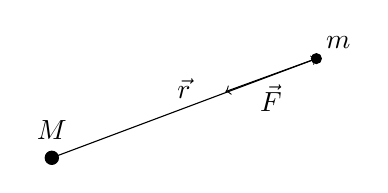
\begin{tikzpicture}[scale=1.05]
\draw[fill=black] (0,0) circle (0.08);
\node[above] at (0,0.1) {$M$};
\draw[fill=black] (3.2,1.2) circle (0.06);
\node[above right] at (3.2,1.2) {$m$};
\draw[->] (0,0) -- (3.2,1.2) node[midway, above] {$\vec r$};
\draw[->] (3.2,1.2) -- (2.1,0.8) node[midway, below] {$\vec F$};
\end{tikzpicture}
\caption{Clean reconstruction of the two-body geometry. The radial vector points from the source mass \(M\) to the test mass \(m\), while the gravitational force points inward, opposite to \(\vec r\).}
\end{figure}

\subsection{Question \& Answer}

\paragraph{Equal forces, unequal accelerations.}
If the forces on the Earth and on the falling body are equal and opposite, why does the Earth barely accelerate while the body accelerates strongly?

Because Newton's equation has two ingredients:
\[
\vec a = \frac{\vec F}{m}.
\]
For the same force, the larger mass has the smaller acceleration. Newton's third law gives equality of forces, not equality of accelerations.

\paragraph{Why the inverse-square law?}
The lecture's historical answer runs through Kepler. For circular motion of radius \(r\) and angular frequency \(\omega\), the inward acceleration is
\begin{equation}
a_{\mathrm{circ}}=\omega^2 r.
\end{equation}
If the force per unit mass behaves as \(f(r)\propto 1/r^2\), then
\begin{equation}
\omega^2 r \propto \frac{1}{r^2},
\qquad\text{so}\qquad
\omega^2\propto \frac{1}{r^3}.
\end{equation}
Since \(T=2\pi/\omega\), we obtain
\begin{equation}
T^2\propto r^3.
\end{equation}
This is Kepler's famous relation between period and orbital radius. In the lecture this is not presented as a full historical proof, but as the right Newtonian clue: Kepler's law strongly points toward the inverse-square force, and the inverse-square law is then the law that extends correctly beyond perfect circles to elliptical orbits.

\section{Many-Body Gravity and the Gravitational Field}

Now replace the two-body problem by a whole assembly of particles. In Newtonian gravity the total force on a given particle is the vector sum of the pairwise forces exerted by all the others. The lecture arrives at this on the blackboard, including a live correction of the sign convention when a student notices that the interparticle vector has been taken in the wrong direction. It is better to clean the convention once and for all.

Let \(\vec r_i\) be the position of the \(i\)-th particle, and let \(\vec r_j-\vec r_i\) point from particle \(i\) to particle \(j\). Then the force on the \(i\)-th particle is
\begin{equation}
\vec F_i=\sum_{j\ne i} G\,m_i m_j\,
\frac{\vec r_j-\vec r_i}{|\vec r_j-\vec r_i|^3}.
\end{equation}
Every term is attractive because every term points toward the corresponding source particle \(j\).

Combining this with Newton's equation \(\vec F_i=m_i\vec a_i\) gives
\begin{align}
m_i\vec a_i
&=\sum_{j\ne i} G\,m_i m_j\,
\frac{\vec r_j-\vec r_i}{|\vec r_j-\vec r_i|^3}, \\
\vec a_i
&=\sum_{j\ne i} G\,m_j\,
\frac{\vec r_j-\vec r_i}{|\vec r_j-\vec r_i|^3}.
\end{align}
Once again the mass of the particle whose motion we are following cancels. The acceleration of particle \(i\) depends on the other masses, but not on \(m_i\) itself.

This is the natural place in the lecture to introduce the gravitational field. One imagines adding a very light extra particle, a \emph{test particle}, so light that it does not appreciably influence the motion of the rest. Then one asks how that test particle would accelerate at the point where it is placed.

\begin{definition}
The gravitational field at a point \(\vec x\) is the acceleration of a sufficiently light test particle placed at \(\vec x\).
\end{definition}

If the source masses are at positions \(\vec r_j\), then a clean Newtonian expression is
\begin{equation}
\vec g(\vec x)=\sum_j G\,m_j\,
\frac{\vec r_j-\vec x}{|\vec r_j-\vec x|^3}.
\end{equation}
The lecture temporarily denotes this acceleration field by \(\vec A\). We will reserve \(\vec A\) for the generic vector field used in the next section and keep \(\vec g\) for gravity itself.

There is an important conceptual distinction here. The formula above is a force law if all positions are known. But once all the particles are allowed to move, each one changes the motion of the others, and the full many-body dynamics becomes complicated. What the lecture wants at this stage is simpler: the field is the acceleration pattern laid out through space at a given instant.

\section{Tidal Forces and the Limits of Free Fall}

The lecture now returns to the equivalence principle and tightens it. Earlier we said that free fall in a uniform gravitational field is locally indistinguishable from gravity-free motion. Now we must say more carefully where that statement stops being true.

Once the gravitational field depends on position, a large body no longer has all its parts accelerated in exactly the same way. Suppose an absurdly tall person falls feet-first toward the Earth. The feet are closer to the Earth than the head, so the lower parts feel a larger downward acceleration than the upper parts. The body is therefore stretched vertically.

Now rotate the same body so that it lies horizontally. The left side and the right side are at roughly the same distance from the Earth, but the forces are no longer parallel. Each side is pulled radially inward, so the left side is pulled slightly to the right and the right side slightly to the left. The body is therefore compressed horizontally.

This is the Newtonian content of tidal force: neighboring parts of an extended object experience slightly different accelerations and slightly different directions of pull because the field \(\vec g(\vec x)\) varies across the object.

\subsection{Question \& Answer}

If free fall hides gravity, why do sufficiently large falling bodies get stretched and squeezed?

Because free fall hides only the \emph{common} part of the acceleration. If the field were perfectly uniform, every part of the body would share the same motion and nothing internal could reveal gravity. But a real gravitational field is not uniform. Different points of the body sample different values of \(\vec g(\vec x)\), and those differences are precisely the tidal forces.

That is why the lecture keeps both statements. A small enough freely falling object does not notice gravity, because the variation of the field across its size is negligible. A large enough object does notice gravity, because the gradient of the field across its size is no longer negligible. The body is then stretched in one direction and squeezed in another.

This also explains the name. The Moon exerts tidal forces on the Earth: it tends to stretch the Earth--ocean system along the Earth--Moon line and compress it in the transverse directions. The rigid Earth deforms only slightly, but the water responds much more visibly.

\section{Divergence and Gauss's Theorem}

After the break the lecture makes a clean mathematical pivot. If the gravitational field is now regarded as a vector field spread through space, we need a way to describe its local structure. The first tool is divergence.

The blackboard frame below preserves the lecture's explicit formula.

\begin{figure}
\centering

\includegraphics[width=0.84\textwidth]{lecture_01_figure_05.png}
\caption{The blackboard definition of divergence. The important distinction is between the vector field \(\vec A\) and the scalar quantity \(\nabla\cdot\vec A\).}
\end{figure}

Let \(\vec A(\vec x)\) be a vector field with components \(A_x,A_y,A_z\). The lecture defines its divergence by
\begin{equation}
\nabla\cdot\vec A
=
\partial_x A_x+\partial_y A_y+\partial_z A_z
=
\frac{\partial A_x}{\partial x}
+\frac{\partial A_y}{\partial y}
+\frac{\partial A_z}{\partial z}.
\end{equation}
This is not a vector. It is a scalar. The field \(\vec A\) may point somewhere; the divergence measures, at a point, whether the field is locally spreading out or converging in.

To make this intuitive, Susskind turns to a water-flow analogy. We imagine a shallow lake with fixed depth, or more generally an incompressible fluid whose density is kept fixed. If water is being pumped in from below at a point, the velocity field spreads outward from that point; the divergence is positive there. If water is being removed, the field converges inward; the divergence is negative there. The analogy is deliberately simplified. It is meant to isolate source and sink behavior, not to develop the full mechanics of compressible fluids.

The lecture's schematic arrow-field is preserved below.

\begin{figure}
\centering

\includegraphics[width=0.50\textwidth]{lecture_01_figure_06.png}
\caption{Arrow-field sketch used in the lecture to explain local divergence. The key idea is to compare what flows into and out of a small region placed between neighboring arrows.}
\end{figure}

\begin{figure}
\centering
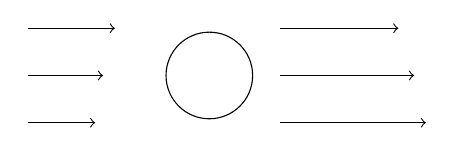
\begin{tikzpicture}[scale=1.0]
\draw[->] (-2.3,1.0) -- (-1.2,1.0);
\draw[->] (-2.3,0.4) -- (-1.35,0.4);
\draw[->] (-2.3,-0.2) -- (-1.45,-0.2);

\draw[->] (0.9,1.0) -- (2.4,1.0);
\draw[->] (0.9,0.4) -- (2.6,0.4);
\draw[->] (0.9,-0.2) -- (2.75,-0.2);

\draw (0.0,0.4) circle (0.55);
\end{tikzpicture}
\caption{Reconstruction of the control-region picture described in the lecture. More field leaves the small circle on the right than enters from the left, so the region has positive divergence.}
\end{figure}

The second mathematical tool is the theorem that relates local divergence to total flux through a boundary.

\begin{theorem}[Gauss's theorem]
For a vector field \(\vec A\),
\begin{equation}
\int_V (\nabla\cdot\vec A)\,dV
=
\oint_{\partial V} A_\perp\,d\sigma
=
\oint_{\partial V} \vec A\cdot \hat n\,d\sigma.
\end{equation}
\end{theorem}

The meaning is direct. The integral on the left adds up all sources and sinks inside the region \(V\). The integral on the right adds up the net outward flow through the boundary \(\partial V\). Only the normal component contributes; tangential flow slides along the boundary and does not leave the region.

For the lecture, this theorem is not an isolated vector-calculus fact. It is the central bridge back to gravity.

\section{Spherical Symmetry, Newton's Theorem, and Shells}

Now we apply Gauss's theorem to a spherically symmetric source. Suppose the divergence of a vector field \(\vec A\) is confined to some finite spherical region. Outside that region the divergence vanishes. Let the total enclosed divergence be
\begin{equation}
Q=\int_V (\nabla\cdot\vec A)\,dV.
\end{equation}
If we draw a larger sphere of radius \(r\) enclosing the source, then \(Q\) does not depend on the size of that larger sphere, because all the source is already inside.

By spherical symmetry, the field outside must be radial and must have the same magnitude everywhere on the Gaussian sphere. Therefore the flux integral collapses to
\begin{align}
Q
&=
\oint_{\partial V} A_\perp\,d\sigma
=
A(r)\oint_{\partial V} d\sigma \\
&= 4\pi r^2\,A(r).
\end{align}
Hence
\begin{equation}
A(r)=\frac{Q}{4\pi r^2},
\qquad
\vec A(r)=\frac{Q}{4\pi r^2}\hat r.
\end{equation}
This is the lecture's clean derivation of a \(1/r^2\) field from spherical symmetry plus Gauss's theorem.

For gravity the sign must be reversed. The physical gravitational field points inward, not outward. Thus the gravitational analog of a positive source is really a convergence. For a point mass \(M\) we therefore write
\begin{equation}
\vec g(r)=-\frac{GM}{r^2}\hat r.
\end{equation}

This leads immediately to Newton's theorem.

\begin{proposition}[Newton's theorem]
Outside a spherically symmetric mass distribution, the gravitational field is exactly the same as that of a point mass with the same total mass concentrated at the center.
\end{proposition}

That statement is stronger than it may first appear. It says that the exterior field does not care whether the mass is concentrated at a point, spread out smoothly, denser near the center, or denser near the surface. As long as the distribution is spherically symmetric and we stand outside it, only the total mass matters.

There is, however, an equally important limitation. This is an exterior theorem. Once we move inside the mass distribution, we are asking a different question. The lecture makes this point with the mine shaft. Near the center of the Earth the force is certainly not what it would be if the entire Earth's mass were concentrated at the center. The exterior theorem does not extend unchanged to interior points.

\begin{figure}
\centering
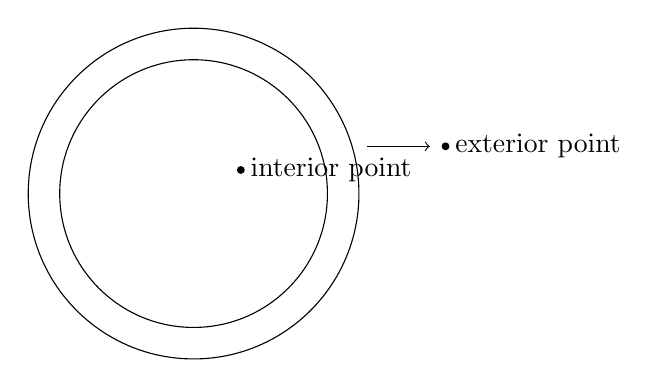
\begin{tikzpicture}[scale=1.0]
\draw (0,0) circle (1.7);
\draw (0,0) circle (2.1);
\fill (0.6,0.3) circle (0.05);
\node[right] at (0.6,0.3) {interior point};
\fill (3.2,0.6) circle (0.05);
\node[right] at (3.2,0.6) {exterior point};
\draw[->] (2.2,0.6) -- (3.0,0.6);
\end{tikzpicture}
\caption{A spherical shell. Outside the shell, the field is the same as that of a point mass at the center. Inside the shell, the field vanishes.}
\end{figure}

\subsection{Question \& Answer}

Why is the field outside a spherical body point-mass-like, while the field inside a spherical shell vanishes?

Outside the body, the answer is Gauss plus symmetry. A Gaussian sphere enclosing the entire spherically symmetric source sees only the total enclosed mass. The flux is therefore fixed. Since the field has the same magnitude everywhere on that sphere and points radially, the only possibility is the \(1/r^2\) field of a point mass with the same total mass.

Inside a hollow spherical shell, the answer is even sharper. A Gaussian surface lying entirely inside the shell encloses no source at all. Therefore the enclosed divergence is zero, and the net flux through the Gaussian surface is zero. But by symmetry there is no preferred interior direction. The only field compatible with zero enclosed source and full spherical symmetry is
\[
\vec g_{\text{inside shell}}=0.
\]

The lecture rightly lingers here. This is not just a clever exercise. It is the theorem that makes the Newtonian treatment of planets possible. A spherical planet may be treated, from outside, as though all its mass were concentrated at the center.

\section{Summary}

The lecture begins with the most elementary Newtonian formula and ends with the shell theorem, but the path is very deliberate. First we learn that gravity is special because its force is proportional to the same mass that appears in Newton's law; in a uniform field the mass cancels, and free fall becomes universal. Then we replace the flat-Earth approximation by Newton's inverse-square law, sharpen that law into vector form, and generalize it to many bodies. The motion of a test particle again ignores its own mass, which leads naturally to the idea of a gravitational field.

Finally, once the field is treated as a vector field in space, divergence and Gauss's theorem explain why spherical symmetry produces a \(1/r^2\) law and why spherical shells are so remarkable. That is the real payoff of the lecture: already within Newtonian gravity, the mathematics begins to organize itself in a way that points toward geometry.